Salmon have an optimal temperature range for the rate at which they grow, migrate, and reproduce. 
If the temperature of their environment goes outside of that range, then salmon may change their spawning location or time frame of migration~\cite{ADFG-optimal}.
If they do not take either of those options, then they may fatigue and die before reaching their spawning location \cite{ADFG-optimal, ADFG-critical}.
So, when temperatures reach a critical point, mortality rates increase significantly, which consequently decreases their growth rate \cite{ADFG-optimal}.
The purpose of this section is to use salmon's mortality rate during spawning migration at different temperatures to approximate a growth rate function, $R(T)$, that is dependent upon temperature.
While there is little research that scientifically describes the effects of salmon population growth at each temperature, there are reports that estimate the optimum temperature range for maximum survival and critical points where survival becomes unlikely.
Dr. Phyllis Weber Scannell wrote an article in 1992 for the Alaskan Department of Fish and Game (ADFG) about the optimal temperature ranges for cold water fish.
In this article, she highlights the optimal range as well as the critical high temperature of sockeye salmon in Alaska~\cite{ADFG-optimal}.
Also, Katherine Carter has published an article that suggests temperatures below $2^{\circ}$C will result in a high mortality rate~\cite{carter2005effects}.\\
% Also, Katherine Carter published an article that we use to suggest that temperatures below $2^{\circ}$C will result in a high mortality rate~\cite{carter2005effects}.\\
\begin{table}[H]
\rowcolors{2}{white!40}{lightgray!40}
    \centering
    \caption{Optimal Temperature Range For Pacific Sockeye Salmon}\label{tab:optimaltemp}
    \vspace{.75cm}
    \begin{tabular}{|c|c|c|c|}
    \hline
         \textbf{Species} & \textbf{Optimal ($^{\circ}$C)} & \textbf{Low ($^{\circ}$C)} & \textbf{High ($^{\circ}$C)}\\
         \hline
         Sockeye & $11-14$ & $<2$ & $>22.2$\\
         \hline
    \end{tabular}
    \vspace{1ex}
    
    {\singlespacing
    % \raggedright 
    *The optimal, critical high and low temperature range for the sockeye salmon species in Alaska \cite{ADFG-optimal, carter2005effects}.\par}
\end{table}
As Dr. Scannel's report states, each researcher estimates slightly different temperature ranges due to a multitude of variables such as acclimation, age, size, genetic strain, and physiological conditions of the fish~\cite{ADFG-optimal}.
That being said, we use \tablename~\ref{tab:optimaltemp} to help fit a curve that best illustrates the impact of temperature on the proportion of salmon that survive their spawning migration.
Now, Katherine Carter's article explains that at these critical points the population could have a mortality rate of 50\%~\cite{carter2005effects}.
% Now, Katherine Carter's article explains that at these critical points the population would have a 50\% mortality rate~\cite{carter2005effects}.
So, we estimate that under ideal conditions and optimal temperatures, 100\% of the salmon population would survive the spawning migration to reproduce, and at critical temperatures, only 50\% would survive.
From \tablename~\ref{tab:optimaltemp} the optimal temperature range is $11-14^{\circ}$C and the critical temperature points are at $2^{\circ}$C and $22.2^{\circ}$C, which can be observed on the graph below.
\begin{figure}[H]
    \centering
    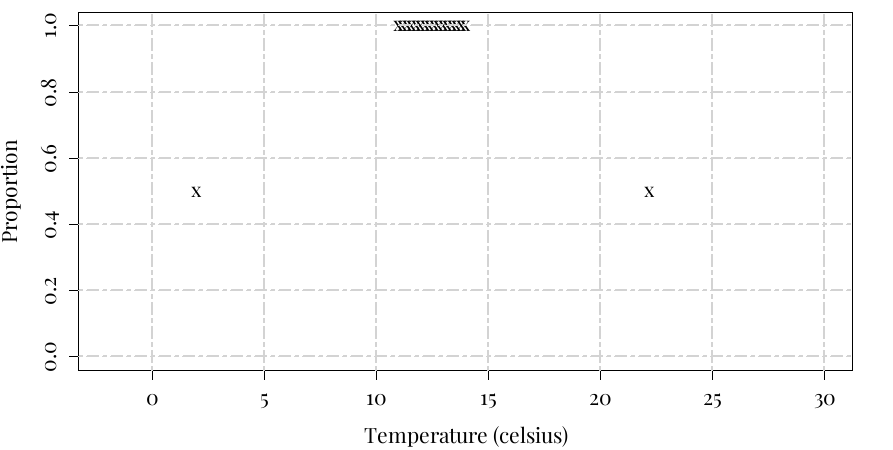
\includegraphics[width=14cm]{Pictures/Salmon Pop/salmon repo model/proportion survival.png}
    \caption{\singlespacing
    Scatter plot of the survival rates in the optimal temperature range and at the critical temperature points.}
    \label{fig:reproductionpoints}
\end{figure}
Given that the width of the optimal range is rather large, developing a function to approximate these data points will be rather difficult.
The proportion of salmon surviving spawning migration cannot drop below 0, which implies that we should be looking at a function similar to the one displayed below,
\begin{equation}\label{eq:repogeneral}
    P(T) = \frac{1}{1+c(T-T_{opt})^p}, \quad p\; \epsilon\; 2\mathbb{N},
\end{equation}
where $P(T)$ estimates the proportion of salmon that will survive spawning migration at a given temperature, $T$, in Celsius, and $T_{opt}$ is the average of the optimal temperature range, $12.5^{\circ}$C. 
The power of the binomial, $p$, controls the average rate of change of the proportions, and $c$ is a constant that will be calculated to stretch or compress the function horizontally.
Now, we get the graph below by setting the parameters $p=2$ and $c=1$ as a starting point for the function above.
\begin{figure}[H]
    \centering
    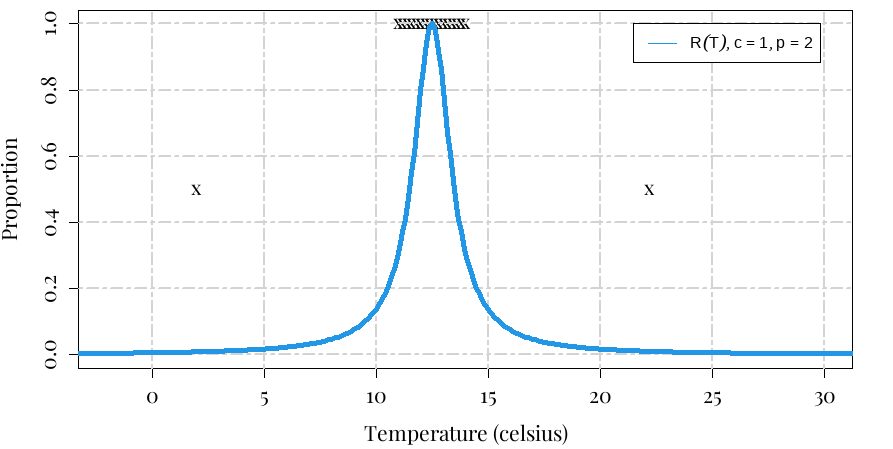
\includegraphics[width=14cm]{Pictures/Salmon Pop/salmon repo model/Repo F2 c1.png}
    \caption{\singlespacing
    Plot of the proportion function, where $c=1$ and $p=2$.}
    \label{fig:reporductioncurve2c1}
\end{figure}
The main issue with these parameters is that the peak of the curve is too narrow to represent the optimal range well, and the curve is too far away from the critical temperature points, $(2,0.5)$ and $(22.2,0.5)$. 
From the graph above, the survival proportion of migrating salmon at the limits of their optimal temperature range is $P(T=11)=P(T=14)\approx0.31$, which is a major deviation from the proposed survival proportion.
So, by adjusting the parameter $c$, we can stretch the function to better fit the survival proportions for the critical and optimal temperatures.
This can be done by taking the average of the distances from $T_{opt}$ to the critical temperatures, as shown below,
\[
Avg = \frac{|T_{opt}-2| + |T_{opt}-22.2|}{2} = 10.1.
\]
From here we can set $P(T)=0.5$ and $T-T_{opt}=Avg=10.1$ and solve for $c$,
\[
c = \frac{1-P(T)}{P(T)(T-T_{opt})^2} = \frac{1-0.5}{0.5(10.1)^2} = \frac{1}{10.1^2} = \frac{1}{102.1}\approx0.01.
\]
Now, plotting $P(T)$ with parameters $p=2$ and $c=0.01$ produces the plot below.
\begin{figure}[H]
    \centering
    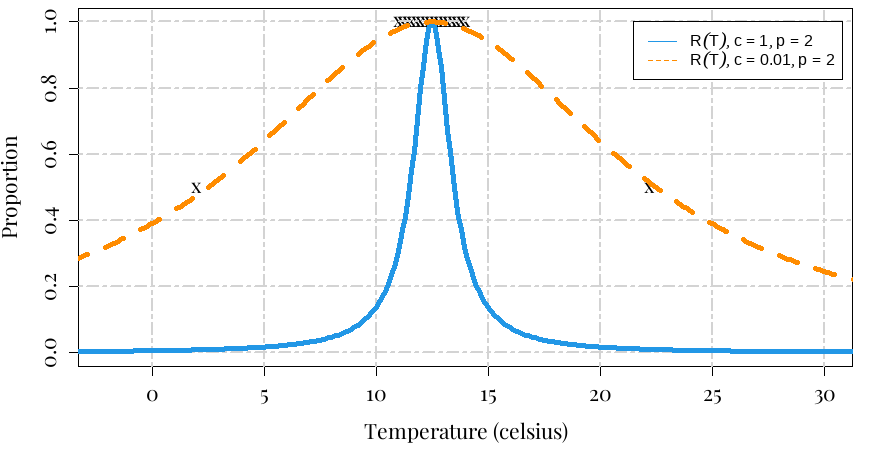
\includegraphics[width=14cm]{Pictures/Salmon Pop/salmon repo model/Repo c1 and c01.png}
    \caption{\singlespacing
    Compares the plots of the proportion function, where $c=1$ and $c=0.01$, but $p=2$ remains the same.}
    \label{fig:reporductioncurve2c1c01}
\end{figure}
From the figure above, the low and high critical temperature points are better represented with the new parameter, $c=0.01$.
However, at the limits of the optimal temperature range, the survival proportion is $0.978$, which should be closer to 1.
This can be resolved by changing the power of the binomial, $p=2$, in \equationautorefname~\eqref{eq:repogeneral} to $p=4$, which will widen the curve while maintaining a steep descent as the temperature escapes the optimal region.
So, substituting the new parameters, $c=0.01$, and $p=4$, the graph below is produced.
\begin{figure}[H]
    \centering
    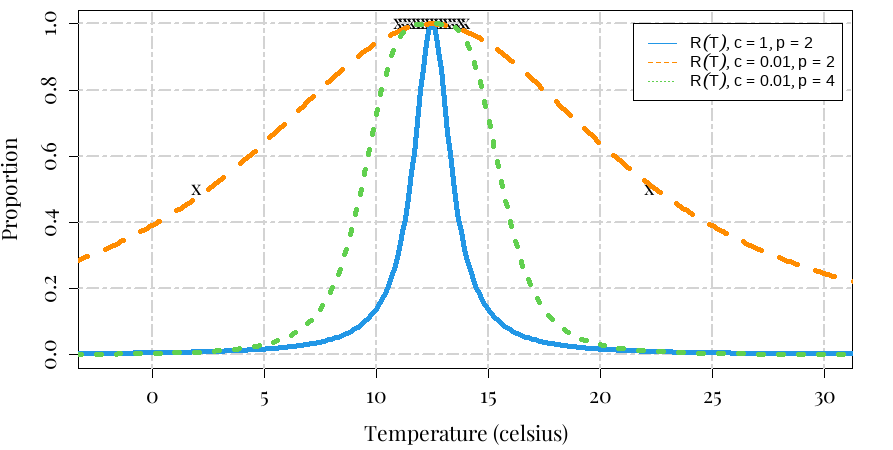
\includegraphics[width=14cm]{Pictures/Salmon Pop/salmon repo model/Repo c1 c01 p4 c01.png}
    \caption{\singlespacing
    Compares the plots of \figureautorefname~\ref{fig:reporductioncurve2c1c01} with the plot of the proportion function, where $c=0.01$ and $p=4$.}
    \label{fig:reproductioncurve2_4_c01}
\end{figure}
With this figure, the representation of the optimal range is better, but the proportions of salmon survival decrease significantly as $T$ approaches the limits of the optimal range.
Also, the survival proportions at the critical temperatures are far from the points, $(2,0.5)$ and $(22.2,0.5)$.
To resolve this issue, we can repeat the same process as earlier to select a new $c$ value that accurately reflects the proportions at the optimal and critical temperatures.
As a result, the graph below is produced by substituting the new parameter $c=10^{-4}$ into the proportion function.
\begin{figure}[H]
    \centering
    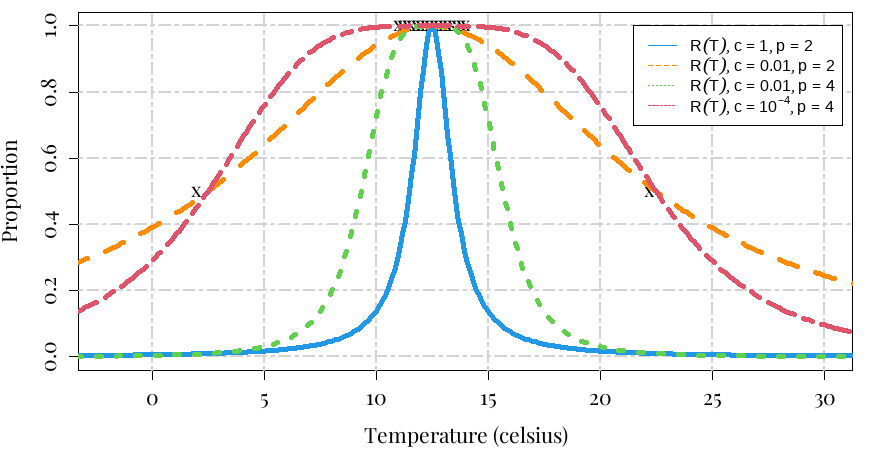
\includegraphics[width=14cm]{Pictures/Salmon Pop/salmon repo model/Repo_all.png}
    \caption{\singlespacing
    Compares the plots of \figureautorefname~\ref{fig:reproductioncurve2_4_c01} with the plot of the proportion function, where $c=10^{-4}$ and $p=4$.}
    \label{fig:reproductioncurve4}
\end{figure}
The parameters, $c=10^{-4}$ and $p=4$, offer a better fit, with the survival proportion being $0.9995$ at the optimal temperature limits and $P(2) \approx 0.45$ and $P(22.2) \approx 0.53$.
By fixing $c=10^{-4},\ p=4$ and $T_{opt}$ in \equationautorefname~\eqref{eq:repogeneral}, we get
\begin{equation}\label{eq:SurvivalProportionFun}
    P(T) = \frac{1}{1+c(T-T_{opt})^p} = \frac{1}{1+10^{-4}(T-12.5)^4},
\end{equation}
where P(T) represents the proportion of salmon that survive spawning migration with respect to temperature.  
During the salmon migration of 2004, Weaver Creek sockeye salmon experienced a drastic rise in water temperature, which resulted in a higher than usual mortality rate~\cite{farrell2008pacific}.
According to Anthony P. Farrell, temperatures were around $20.4^{\circ}$C and 30\% of the salmon population did not make it to the spawning location due to the excessive heat~\cite{farrell2008pacific}.
Using \equationautorefname~\eqref{eq:SurvivalProportionFun}, we get $P(20.4)=0.7197$.
Therefore, we estimate a 72\% survival rate, or a mortality rate of approximately 28\%, for the salmon migrating to their spawning locations, which is close to Anthony P. Farrell's estimation of 30\%.

Looking back, the growth rate, $r_x=\ln{(0.32*5)}$, was estimated when temperatures were ideal, or in the optimal range, so combining the proportion function with the current growth rate, we get the function below,
% \begin{equation}\label{eq:RepoFun}
%     R(T) = 0.32*5*P(T)) = \frac{0.32*5}{1+c(T-T_{opt})^4},
% \end{equation}
\begin{equation}\label{eq:RepoFunLog}
    R(T) = \ln(0.32*5*P(T))  = \ln{\left(\frac{0.32*5}{1+c(T-T_{opt})^4}\right)},
\end{equation}
where $c=10^{-4}$, $T_{opt}=12.5^{\circ}$C, and $T$ is temperature.
% Notice, the proportion function, $P(T)$, is inside the natural log. 
% This is because we want the proportion of salmon that survived the migration after escaping the harvest, which is the same reasoning used when deriving \equationautorefname~\eqref{eq:fishexpbase5}.
Lastly, we will replace the growth rate, $r_x$, with the growth rate function, $R(T)$, in \equationautorefname~\eqref{eq:fishlogistic} to get the below equation,
\begin{equation}\label{eq:salmonlogisticrepo} 
    \frac{dx}{dt} =
    R(T)x\left(1-\frac{x}{K_x}\right).
\end{equation}
To see the effect of temperature on the salmon population, we will compare \equationautorefname~\eqref{eq:salmonlogisticrepo} at different temperatures.
\begin{figure}[H]
    \centering
    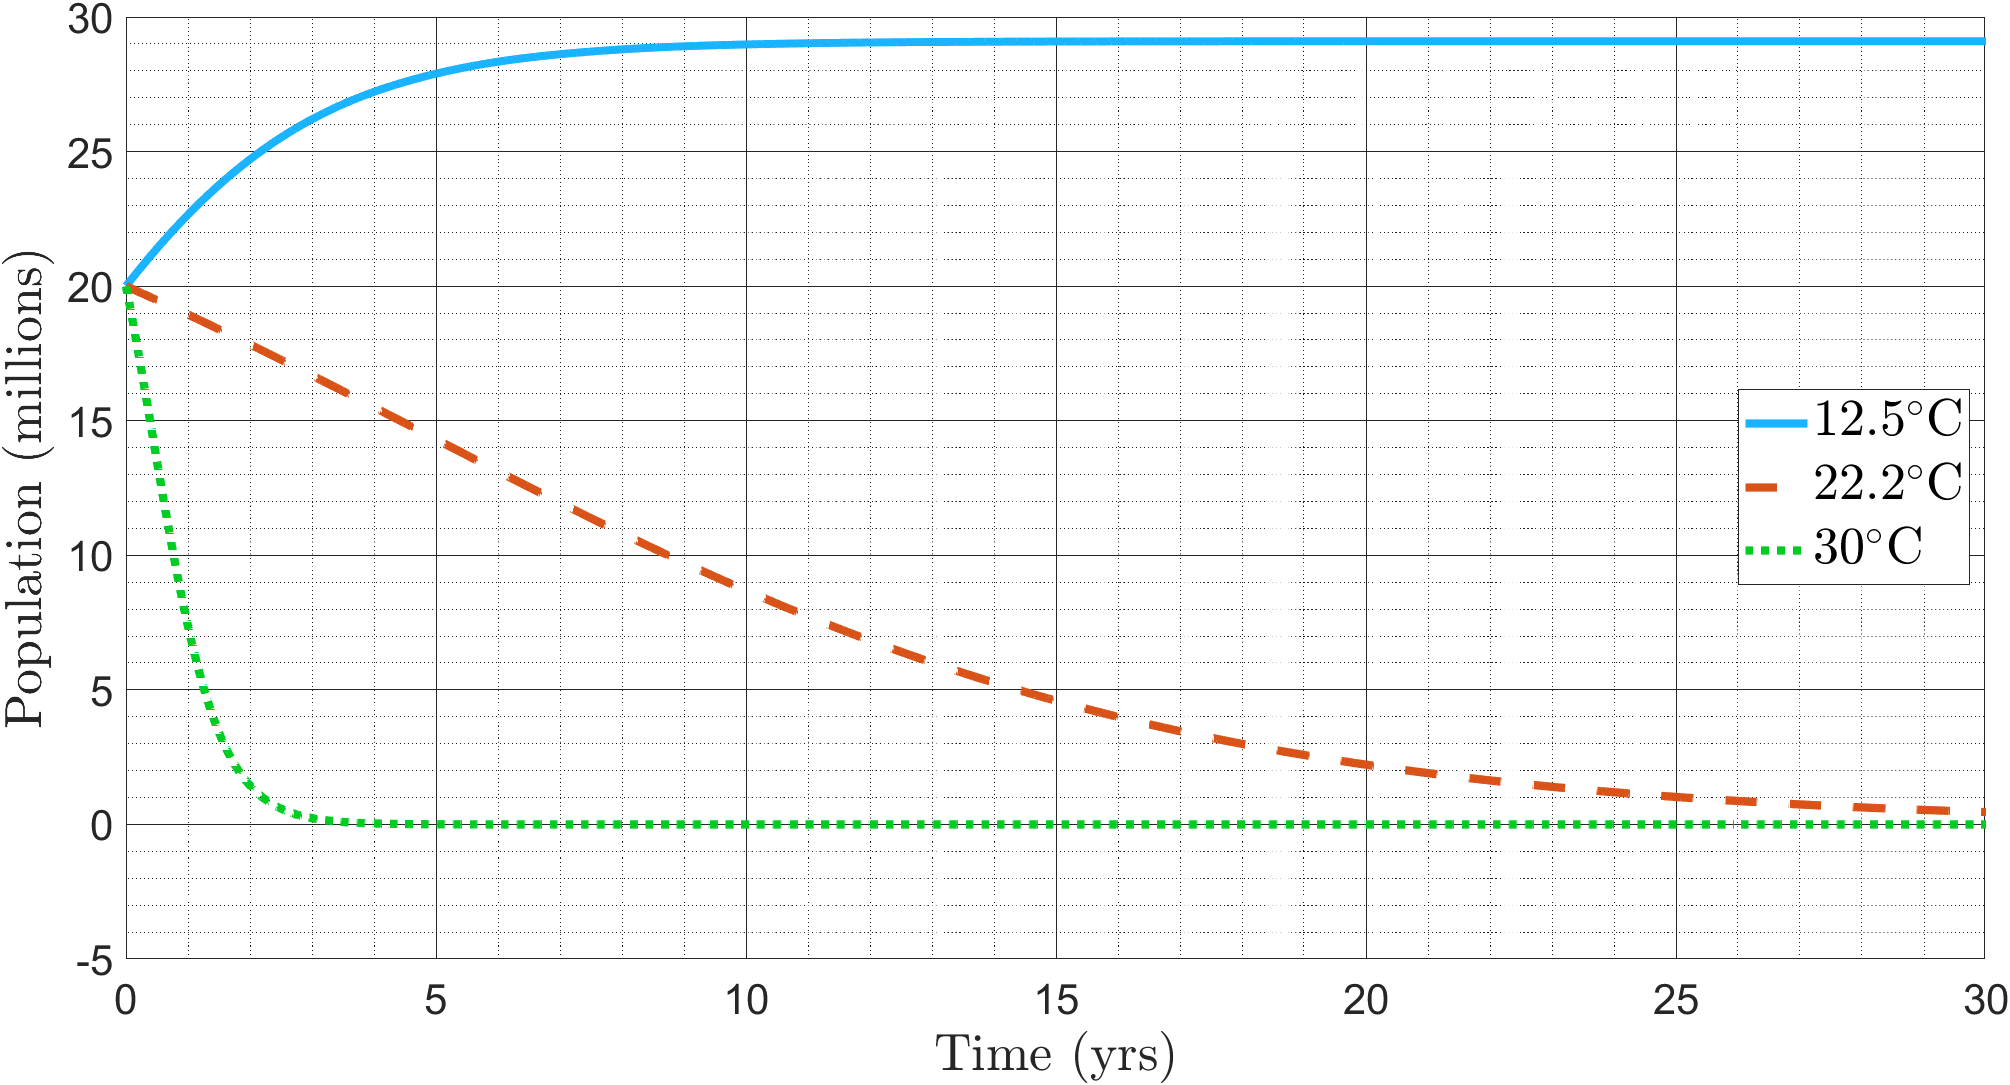
\includegraphics[width=14cm]{Pictures/Salmon Pop/salmon repo model/Salmon at 3 dif temps.png}
    \caption{\singlespacing
    Plot of the salmon logistic growth model using the growth rate function, \equationautorefname~\eqref{eq:salmonlogisticrepo}, at 3 different temperatures.}
    \label{fig:salmonrepocomparison}
\end{figure}
Notice, at the optimal temperature, $T=12.5^{\circ}$C, the curve is the same as in \figureautorefname~\ref{fig:salmnologistic} because $R(12.5) = r_x = 0.47$. 
As the temperature moves further away from the optimal temperature, the reproduction of salmon is negatively affected, resulting in a decay rate, which can be observed in the middle and bottom curves.
When $T=22.2^{\circ}$C the growth rate is $R(22.2) = -0.1641$, which is explains why the population is decreasing over time.
Notice, as the temperature moves drastically far away from the optimal temperature, $T=30^{\circ}$C, the growth rate changes to $R(30)=-1.8698$, causing the population to die off in about 5 years.
By replacing the growth rate of salmon with a function dependent upon temperature, we can see the drastic effects on the salmon population as temperature changes.
